%%%%%%%%%%%%%%%%%%%%%%%%%%%%%%%%%%%%%%%%%
% Beamer Presentation
% LaTeX Template
% Version 1.0 (10/11/12)
%
% This template has been downloaded from:
% http://www.LaTeXTemplates.com
%
% License:
% CC BY-NC-SA 3.0 (http://creativecommons.org/licenses/by-nc-sa/3.0/)
%
%%%%%%%%%%%%%%%%%%%%%%%%%%%%%%%%%%%%%%%%%
%----------------------------------------------------------------------------------------
%	PACKAGES AND THEMES
%----------------------------------------------------------------------------------------
% Interessante: 
%https://www.codecogs.com/latex/eqneditor.php?lang=pt-br


\documentclass{beamer}

\usepackage[brazilian]{babel}
\usepackage[utf8]{inputenc}
\usepackage[T1]{fontenc}
\usepackage{colortbl}
\usepackage{mathrsfs}
\usepackage{smartdiagram}
\usepackage{listings}
\usepackage[framed,numbered,autolinebreaks,useliterate]{mcode}
\usepackage{multirow}


\mode<presentation> {

% The Beamer class comes with a number of default slide themes
% which change the colors and layouts of slides. Below this is a list
% of all the themes, uncomment each in turn to see what they look like.

%\usetheme{default}
%\usetheme{AnnArbor}
%\usetheme{Antibes}
%\usetheme{Bergen}
%\usetheme{Berkeley}
%\usetheme{Berlin}
%\usetheme{Boadilla}
%\usetheme{CambridgeUS}
%\usetheme{Copenhagen}
%\usetheme{Darmstadt}
%\usetheme{Dresden}
\usetheme{Frankfurt}
%\usetheme{Goettingen}
%\usetheme{Hannover}
%\usetheme{Ilmenau}
%\usetheme{JuanLesPins}
%\usetheme{Luebeck}
%\usetheme{Madrid}
%\usetheme{Malmoe}
%\usetheme{Marburg}
%\usetheme{Montpellier}
%\usetheme{PaloAlto}
%\usetheme{Pittsburgh}
%\usetheme{Rochester}
%\usetheme{Singapore}
%\usetheme{Szeged}
%\usetheme{Warsaw}

% As well as themes, the Beamer class has a number of color themes
% for any slide theme. Uncomment each of these in turn to see how it
% changes the colors of your current slide theme.

%\usecolortheme{albatross}
%\usecolortheme{beaver}
%\usecolortheme{beetle}
%\usecolortheme{crane}
%\usecolortheme{dolphin}
%\usecolortheme{dove}
%\usecolortheme{fly}
%\usecolortheme{lily}
%\usecolortheme{orchid}
%\usecolortheme{rose}
%\usecolortheme{seagull}
%\usecolortheme{seahorse}
%\usecolortheme{whale}
%\usecolortheme{wolverine}

%\setbeamertemplate{footline} % To remove the footer line in all slides uncomment this line
%\setbeamertemplate{footline}[page number] % To replace the footer line in all slides with a simple slide count uncomment this line

%\setbeamertemplate{navigation symbols}{} % To remove the navigation symbols from the bottom of all slides uncomment this line
}

\usepackage{graphicx} % Allows including images
\usepackage{booktabs} % Allows the use of \toprule, \midrule and \bottomrule in tables

\usepackage{animate}
\usepackage{hyperref}
\usepackage{media9}
\usepackage{listings}
\usepackage{amsmath}
\usepackage[framed,numbered,autolinebreaks,useliterate]{mcode}
\usepackage{mdframed}
\usepackage{tikz}
\usetikzlibrary{arrows.meta}
\tikzset{%
  >={Latex[width=2mm,length=2mm]},
  % Specifications for style of nodes:
         base/.style = {rectangle, rounded corners, draw=black,
                        minimum width=4cm, minimum height=0.7cm,
                        text centered, font=\sffamily},
         activityStarts/.style = {base, fill=blue!30},
         process/.style = {base, minimum width=2.5cm, fill=orange!15,
                          font=\ttfamily},
         ilumina/.style = {base, minimum width=2.5cm, fill=red!55,
                          font=\ttfamily},           
         coord/.style={coordinate, on chain, on grid, node distance=6mm and 25mm},
}

\usetikzlibrary{arrows,shapes,positioning,shadows,trees}

\tikzset{
  basic/.style  = {draw, text width=2cm, drop shadow, font=\sffamily, rectangle},
  root/.style   = {basic, rounded corners=2pt, thin, align=center,
                   fill=green!30},
  level 2/.style = {basic, rounded corners=6pt, thin,align=center, fill=green!60,
                   text width=8em},
  level 3/.style = {basic, thin, align=left, fill=pink!60, text width=6.5em}
}

%----------------------------------------------------------------------------------------
%	TITLE PAGE
%----------------------------------------------------------------------------------------

\logo
{
    
\includegraphics[width=0.6cm,height=0.6cm,keepaspectratio]{UFJF.jpg}~%
}

\title[Aula 1]{Introdução à Pesquisa Operacional} 

\author{\scriptsize Professores André L.M. Marcato, Ivo C.da Silva Jr, Joao A.Passos Filho } % Your name
\institute[UFJF/PPEE]{Universidade Federal de Juiz de Fora \\
	Programa de Pós-Graduação em Engenharia Elétrica \\
	\medskip
	\textit{\href{mailto:andre.marcato@ufjf.edu.br}{andre.marcato@ufjf.edu.br}, \href{mailto:ivo.chaves@ufjf.edu.br}{ivo.junior@ufjf.edu.br},\href{mailto:joao.passos@ufjf.edu.br}{joao.passos@ufjf.edu.br}}
}

%\date{\small \today} % Date, can be changed to a custom date
\date{\small Primeiro Semestre de 2018} % Date, can be changed to a custom date

\hypersetup{
    colorlinks=true,
    linkcolor=gray,
    filecolor=magenta,      
    urlcolor=cyan,
}

\begin{document}

\begin{frame}
\titlepage % Print the title page as the first slide
\begin{figure}[!htb]
\centering
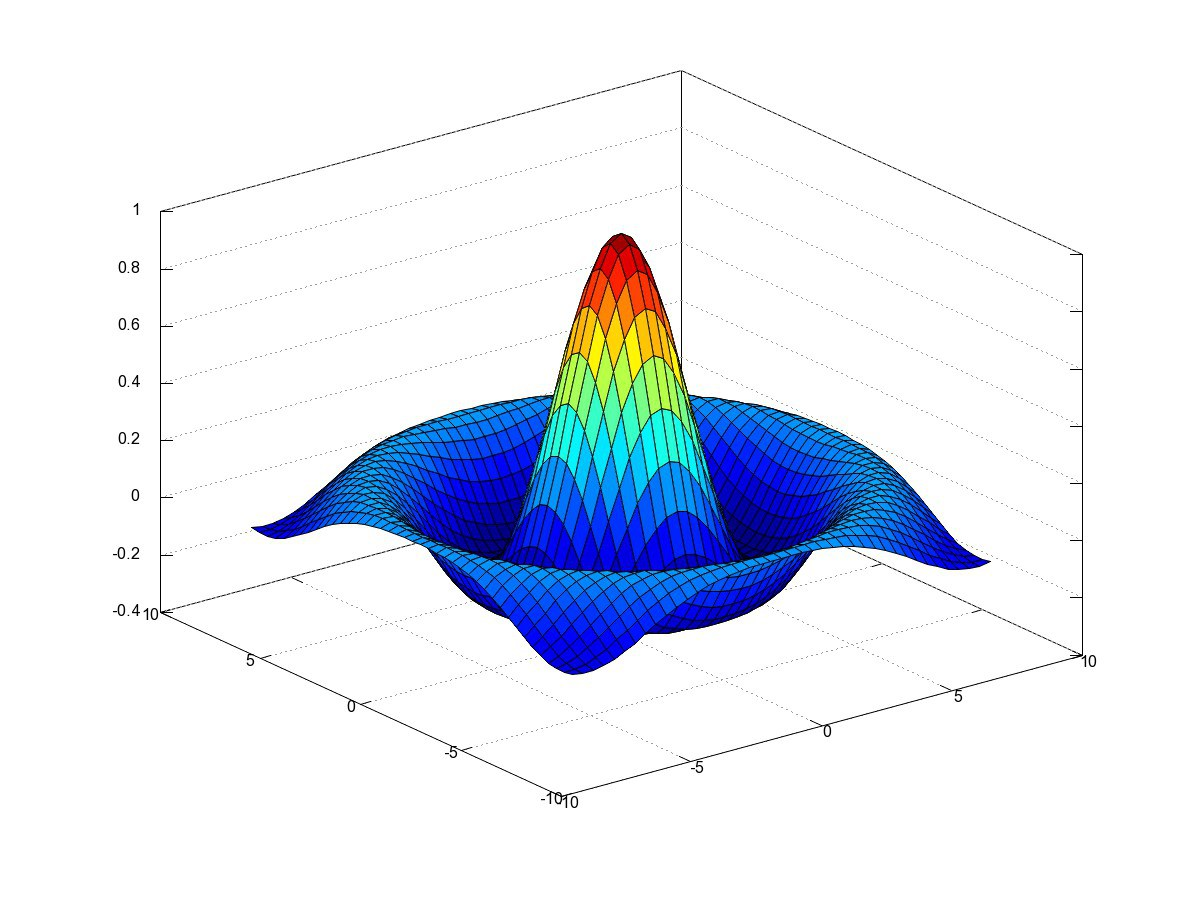
\includegraphics[width=4.0cm, height=2.7cm]{cover.jpg}
%\caption{Ogata - 5a Edicao - Fig. 1.1}
\label{Ogata_1_1}
\end{figure}
\end{frame}

\begin{frame}
\frametitle{Agenda da Apresentação} % Table of contents slide, comment this block out to remove it
\tableofcontents % Throughout your presentation, if you choose to use \section{} and \subsection{} commands, these will automatically be printed on this slide as an overview of your presentation
\end{frame}

%----------------------------------------------------------------------------------------
%	PRESENTATION SLIDES
%----------------------------------------------------------------------------------------

%\include{intro_e_avanco}

\section{Introdução}
\subsection{Pesquisa Operacional}

\begin{frame}
	\frametitle{Pesquisa Operacional}
	\begin{itemize}
	\item 
\includegraphics[width=.7cm,height=.4cm]{portugal.png} \text{  Investigação Operacional}
	\item 
\includegraphics[width=.7cm,height=.4cm]{inglaterra.jpg} \text{  Operational Research}
	\item 
\includegraphics[width=.7cm,height=.4cm]{usa.jpg} \text{  Operations Research}
	\item {Outras Denominações}
		\begin{itemize}
			\item[-] Programação Matemática
			\item[-] Otimização 
		\end{itemize}	
	\end{itemize}
\end{frame}

\begin{frame}
	\frametitle{Principais Sociedades de PO}
	\begin{itemize}
		\item {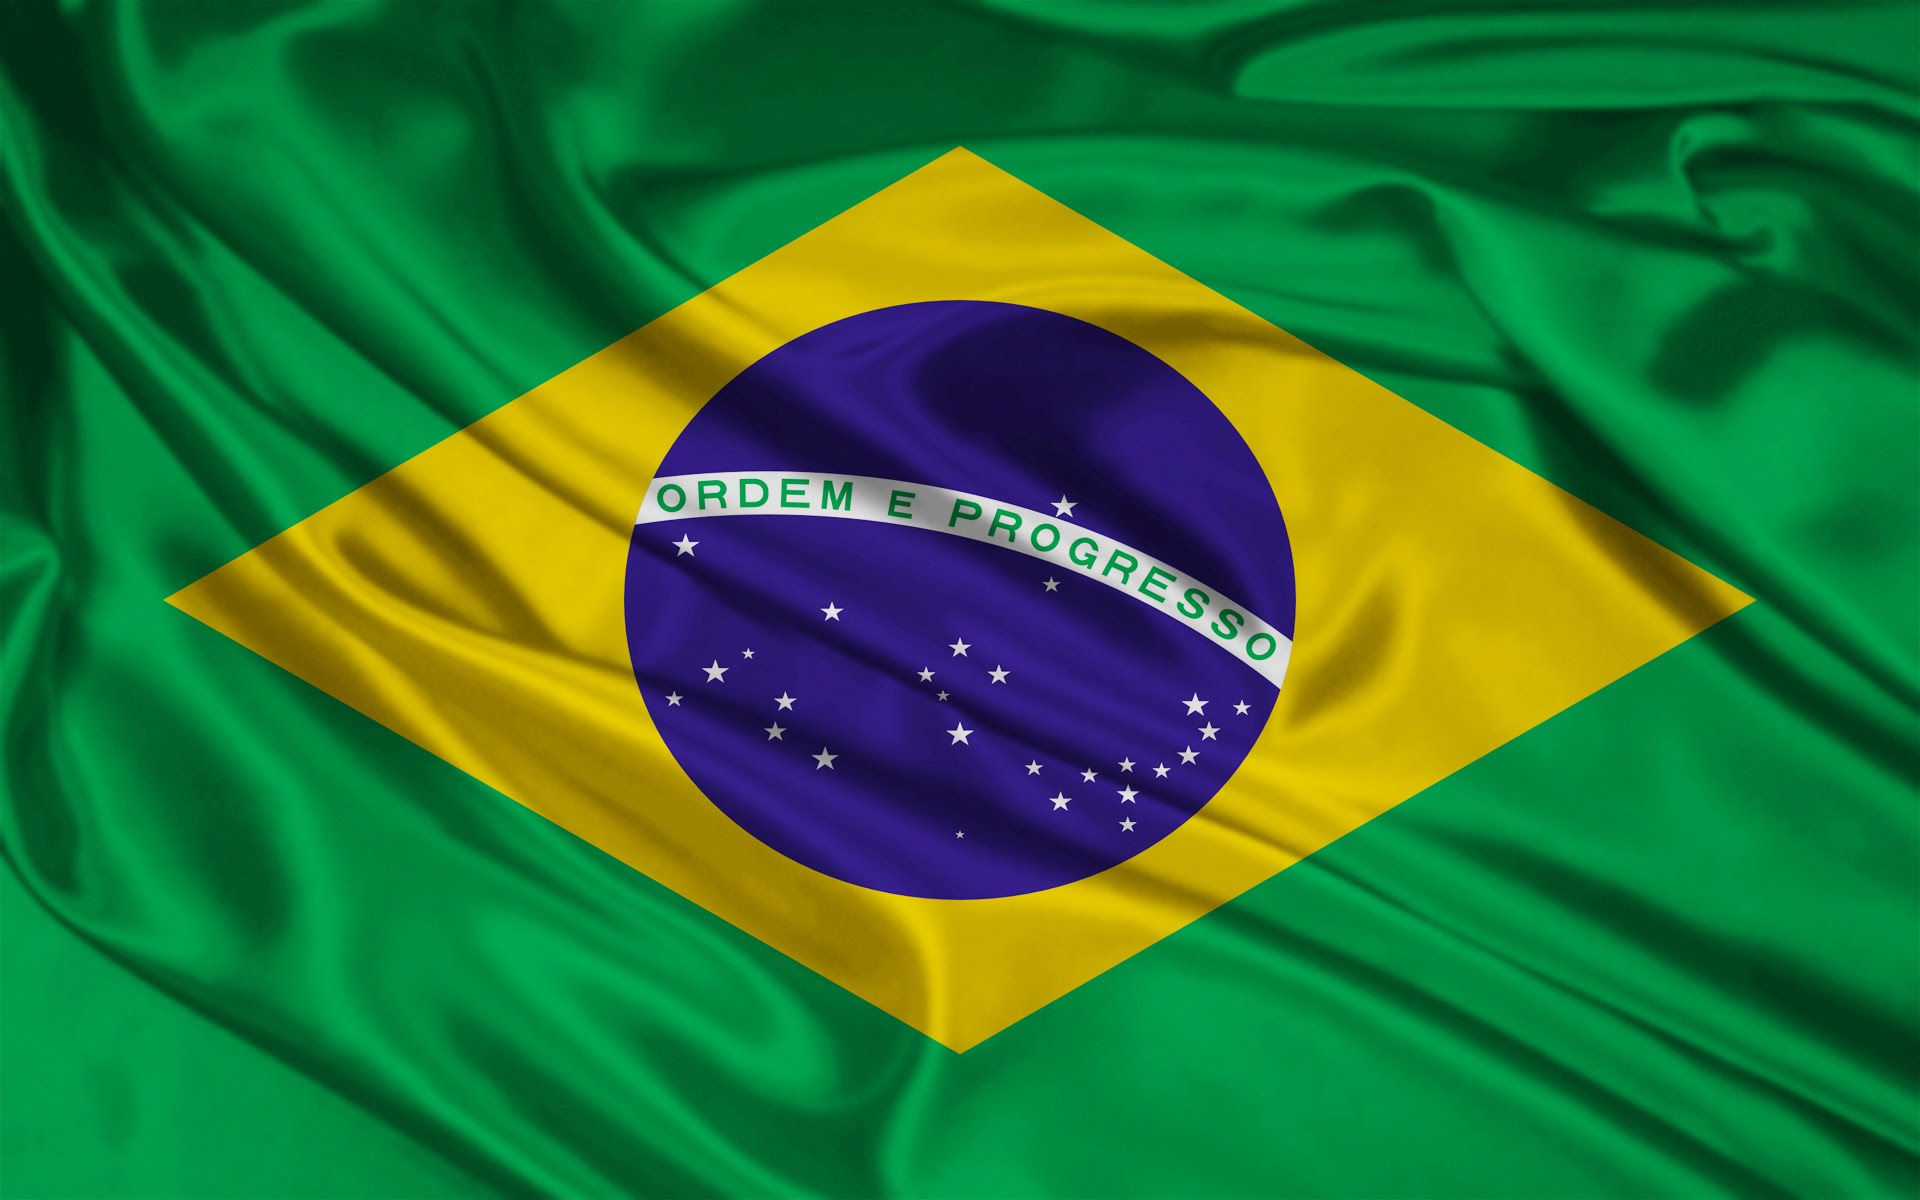
\includegraphics[width=.7cm,height=.4cm]{brasil.jpg}}
			\begin{itemize}
				\item[-] \href{http://www.sobrapo.org.br}{Sobrapo} (Sociedade Brasileira de Pesquisa Operacional) 
			\end{itemize} 
		\item {
\includegraphics[width=.7cm,height=.7cm]{world.png}}
			\begin{itemize}
				\item[-] \href{https://www.informs.org}{INFORMS} (Institute for Operations Research and Management Science)
				\item[-] \href{https://www.euro-online.org/web/pages/1/home}{EURO} (The Association of European Operational Research Societies)
				\item[-] \href{http://apdio.pt/home}{APDIO} (Associação Portuguesa de Investigação Operacional)
				\item[-] \href{http://ifors.org}{IFORS} (International Federation of Operational Research Societies)
				\item[-] \href{http://www-2.dc.uba.ar/alio/}{ALIO} (Assoación Latino-Ibero-Americana de Investigatión Operativa)
			\end{itemize} 	
	\end{itemize}
\end{frame}

\begin{frame}
	\frametitle{O que é otimizar?}
	\begin{figure}
		
\includegraphics[width=3cm,height=3cm]{Pensando.jpg}
	\end{figure}
	\begin{block}{Pergunta: O que é otimizar?}
		\begin{itemize}
			\item[] \textbf{Significado de Otimizar}
			\item[] v.t. Dar a algo (uma máquina, uma empresa, uma situação) um rendimento ótimo, criando-lhe as condições mais favoráveis ou tirando (dele ou dela) o melhor partido possível; tornar (algo) ótimo ou ideal.
		\end{itemize}
	\end{block}	
\end{frame}

\begin{frame}
	\frametitle{O que é otimizar?}
	\begin{figure}
		
\includegraphics[width=3cm,height=3cm]{alvo.png}
	\end{figure}
	\begin{block}{Pergunta: O que é otimizar?}
		\begin{itemize}
			\item[] EXTRAIR A MELHOR SOLUÇÃO POSSÍVEL DE UM DETERMINADO PROBLEMA/SITUAÇÃO
		\end{itemize}
	\end{block}	
\end{frame}

\begin{frame}
	\frametitle{Histórico}
	\centering
	\only<1>
	{
	\begin{figure}
		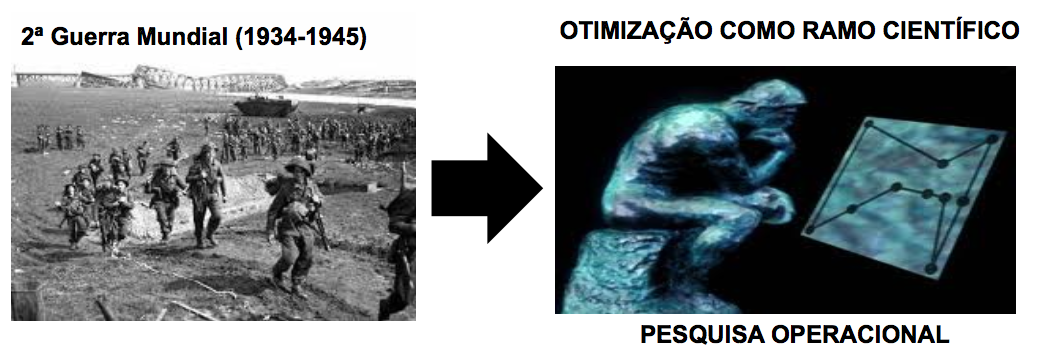
\includegraphics[width=10cm,height=3cm]{seg_guerra.png}
	\end{figure}
	Investigação de forma sistemática e racional dos processos envolvidos na realização de uma atividade produtiva (bélica ou não)
	}
	\only<2>
	{
	\begin{figure}
		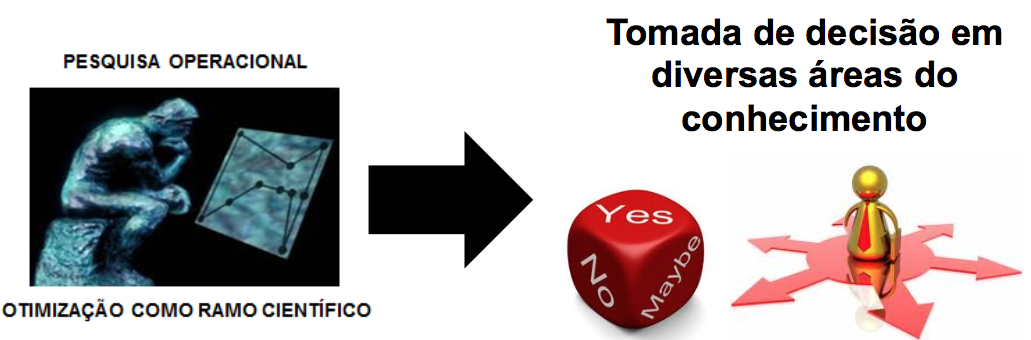
\includegraphics[width=10cm,height=3cm]{ciencia.png}
	\end{figure}
	}
\end{frame}

\begin{frame}
	\frametitle{IFORS 2014 - Technical Program (3 em 3 anos)}
	\centering
	\only<1>
	{
	\begin{itemize}
		\item Railway Scheduling Problems
		\item Routing Problems with Profits and Other Applications
		\item Airline/Airport Optimisation in Operations and Scheduling
		\item Supply Chain Planning
		\item Offshore Upstream Logistics
		\item City Logistic Operations
		\item Models for Gas and Electricity Markets
		\item Energy and Environmental Management
		\item Dynamical Systems and Mathematical Modelling
		\item Optimization Methods for Smartgrid Management
		\item Optimization Methods in Transportation Systems
		\item E muito, muito mais !!!!
	\end{itemize}
	}
	\only<2>
	{
	\begin{figure}
		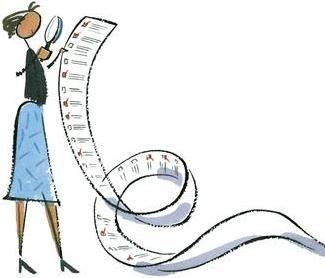
\includegraphics[width=5cm,height=7cm]{lista.jpg}
	\end{figure}
	}
\end{frame}

\section{Modelagem para a Tomada de Decisão}
\subsection{Variáveis de Decisão, Parâmetros, Restrições, Função Objetivo}

\begin{frame}
	\frametitle{Modelagem a Partir de um Sistema Real}
	\centering
	\begin{figure}
		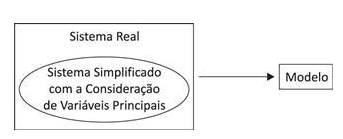
\includegraphics[width=8cm,height=4cm]{Figura_1_3.png}
	\end{figure}
\end{frame}

\begin{frame}
	\frametitle{Modelagem para a Tomada de Decisão}
	\begin{itemize}
	\item[a)] {Variáveis de decisão}
		\begin{itemize}
		\item {Contínuas}
			\begin{itemize}
			\item[-] Pode assumir qualquer valor dentro de um intervalo.  
			\end{itemize}
		\item {Discretas ou Inteiras}
			\begin{itemize}
			\item[-] Ex. Dimensionamento da escala ideal de funcionários por turno de trabalho, Unidades a fabricar de cada tipo de caminhão em uma indústria automobilística 
			\end{itemize}
		\item {Binárias (0 ou 1)}
			\begin{itemize}
			\item[-] Ex. Decidir entre construir ou não uma usina ou linha de transmissão. 
			\end{itemize}		
		\end{itemize}
	\end{itemize}
\end{frame}

\begin{frame}
	\frametitle{Modelagem para a Tomada de Decisão}
	\begin{itemize}
	\item[b)] {Parâmetros}
		\begin{itemize}
		\item[-] São valores previamente conhecidos
		\item[-] Ex. Demanda de cada produto para um problema de mix de produção
		\item[-] Ex. Custo para a produção de determinado tipo de móvel
		\end{itemize}
	\item[c)] {Função objetivo}
		\begin{itemize}
		\item[-] Função matemática que determina o valor alvo que se pretende alcançar
		\item[-] Ex. Minimização do custo de operação de um sistema hidrotérmico
		\item[-] Ex. Maximização do tempo entre a passagem de dois robôs por um ponto em um problema de patrulhamento
		\item[-] Ex. Maximização do fluxo de potência em uma linha de transmissão
		\item[-] Ex. Minimixação da LOLP (Loss of Load Probability) em um problema de confiabilidade
		\end{itemize}	
	\end{itemize}
\end{frame}

\begin{frame}
	\frametitle{Modelagem para a Tomada de Decisão}
	\begin{itemize}
	\item[d)] {Restrições}
		\begin{itemize}
		\item[-] Conjunto de equações ou inequação que as variáveis de decisão devem satisfazer.
		\item[-] Ex. Limitações físicas do sistema
		\item[-] Ex. Capacidade máxima de produção
		\item[-] Ex. Número máximo de colaboradores
		\item[-] Ex. Risco a ser assumido pelo investidor
		\item[-] Canalização: Limites inferiores e superiores das variáveis de decisão.
		\end{itemize}
	\end{itemize}
\end{frame}

\begin{frame}
	\frametitle{Fases do Estudo da Pesquisa Operacional}
	\begin{columns}
		\begin{column}{0.7\textwidth}
			\begin{tikzpicture}[node distance=1.1cm, every node/.style={fill=white, font=\sffamily}, align=center]
				% Specification of nodes (position, etc.)
				\only<1->
				{
					\node (sreal)    [activityStarts]           {Sistema Real};
					\node (defprob)  [process,below of=sreal]   {Definição do Problema};
					\node (modmat)   [process,below of=defprob] {Construção do Modelo Matemático};
					\node (solmod)   [process,below of=modmat]  {Solução do Modelo};
					\node (valmod)   [process,below of=solmod]  {Validação do Modelo};
					\node (impres)   [process,below of=valmod]  {Implementação dos Resultados};
					\node (avafin)   [process,below of=impres]  {Avaliação Final};
					\node (p1)		 [coordinate,left of=defprob,xshift=-2.4cm] {};
					\node (p2)		 [coordinate,left of=defprob,xshift=-2.7cm] {};
					\node (p3)		 [coordinate,right of=modmat,xshift=2.5cm]  {};
					\node (p4)		 [coordinate,right of=modmat,xshift=2.8cm]  {};
					\node (p5)	 	 [coordinate,left of=valmod,xshift=-2cm]    {};
				}
				\only<2>
				{
					\node (defprob)  [ilumina,below of=sreal]   {Definição do Problema};
				}
				\only<3>
				{
					\node (modmat)   [ilumina,below of=defprob] {Construção do Modelo Matemático};
				}
				\only<4>
				{
					\node (solmod)   [ilumina,below of=modmat]  {Solução do Modelo};
				}
				\only<5>
				{
					\node (valmod)   [ilumina,below of=solmod]  {Validação do Modelo};
				}
				\only<6>
				{
					\node (impres)   [ilumina,below of=valmod]  {Implementação dos Resultados};
				}
				\only<7->
				{
					\node (avafin)   [ilumina,below of=impres]  {Avaliação Final};		
				}
				\draw[->]        (sreal)   -- (defprob);
				\draw[->]        (defprob) -- (modmat);
				\draw[->]        (modmat)  -- (solmod);
				\draw[->]        (solmod)  -- (valmod);
				\draw[->]        (valmod)  -- (impres);
				\draw[->]        (impres)  -- (avafin);
				\draw[-]         (modmat)  -| (p1);
				\draw[->]		 (p1)      -- (defprob);
				\draw[-]		 (solmod)  -| (p2);
				\draw[->]		 (p2)	   -- (defprob);
				\draw[-]		 (solmod)  -| (p3);
				\draw[-]		 (valmod)  -| (p4);
				\draw[->]		 (p3)      -- (modmat);
				\draw[->]		 (p4)      -- (modmat);
				\draw[-]		 (impres)  -| (p5);
				\draw[->]		 (p5)      -- (valmod);
			\end{tikzpicture}
		\end{column}
		\begin{column}{0.3\textwidth}
			\only<2>
			{
				\begin{mdframed}[backgroundcolor=red!55] 
						\scriptsize
				        Etapa de definição dos objetivos a serem alcançados e os possíveis caminhos para a solução do modelo.
				\end{mdframed}
			}
			\only<3>
			{
				\centering
				
\includegraphics[width=2.5cm,height=1.5cm]{importante.png}
				\begin{mdframed}[backgroundcolor=red!55]
					Representação do sistema real através da definição de: 
					\scriptsize
					\begin{itemize}
						\item[-] Variáveis
						\item[-] Função objetivo
						\item[-] Equações
						\item[-] Inequações
						\item[-] Tipo Modelo
						\item[-] Tipo Variáveis
					\end{itemize}
				\end{mdframed}
			}	
			\only<4>
			{
				\begin{mdframed}[backgroundcolor=red!55] 
					\scriptsize
					Utilização de diversas técnicas de otimização para a resoluçõa do modelo matemático desenvolvido. Exemplos:
					\begin{itemize}
					\item[-] Programação Linear
					\item[-] Programação Dinâmica
					\item[-] Bat Search Algorithm
					\end{itemize}
				\end{mdframed}
			}
			\only<5>
			{
				\begin{mdframed}[backgroundcolor=red!55] 
					\scriptsize
					Um modelo pode ser considerado válido se conseguir prever com precisão aceitável, o comportamento do sistma real em estudo.
				\end{mdframed}
			}	
			\only<6>
			{
				\begin{mdframed}[backgroundcolor=red!55] 
					\scriptsize
					Detectar e corrigir possíveis mudanças nos valores da nova solução, podendo o modelo ter que ser validado novamente.
				\end{mdframed}
			}		
			\only<7->
			{
				\centering
				\begin{mdframed}[backgroundcolor=red!55] 
					\scriptsize
					Verificar se o objetivo final foi alcançado.
				\end{mdframed}
			}		
			\only<8>
			{
				\centering
				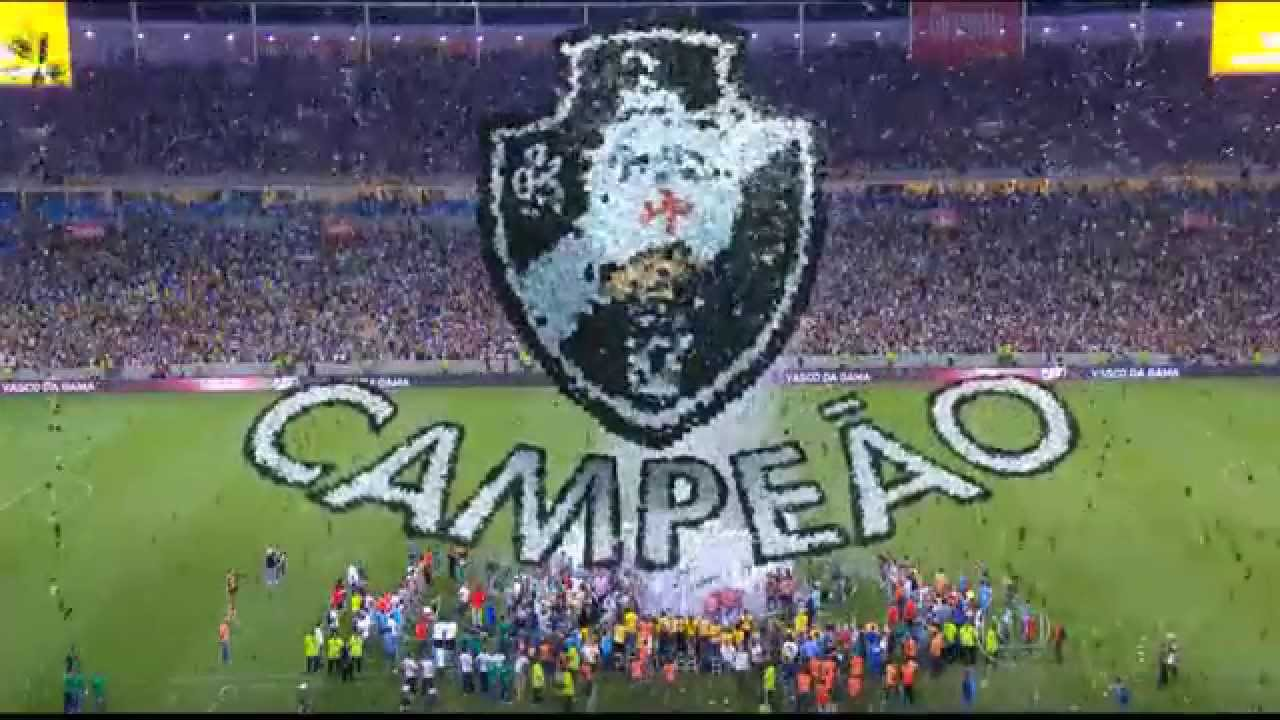
\includegraphics[width=3cm,height=2cm]{vasco.jpg}
			}		
		\end{column}
	\end{columns}
\end{frame}

\begin{frame}
	\frametitle{Tipo Modelo e Tipo Variável}
	\begin{table}[]
		\centering
		\caption{Características dos Problemas de Programação Linear, Não Linear, Binária, Inteira e suas Extensões}
		\scriptsize
		\begin{tabular}{| c | c | }
			\hline
			\hline
			\cellcolor{red!55}Tipo do Modelo  	     & \cellcolor{red!55}Tipo da Variável \\
			\hline
			\hline
			\cellcolor{green!25}Programação Linear (PL) 			   & \cellcolor{green!25}Contínua 	        \\
			\hline
			\cellcolor{cyan!25}Prog.Linear Inteira (PLI) 			   & \cellcolor{cyan!25}Discreta  		    \\
			\hline
			\cellcolor{green!25}Prog.Linear Inteira Mista (PLIM ou PIM)& \cellcolor{green!25}Discreta e Contínua\\
			\hline
			\cellcolor{cyan!25}Prog.Linear Binária (PLB ou PB) 		   & \cellcolor{cyan!25}Binária   	        \\
			\hline
			\cellcolor{green!25}Prog.Linear Binária Mista (PLBM ou PBM)& \cellcolor{green!25}Binária e Contínua \\
			\hline
			\cellcolor{cyan!25}Prog.Não Linear (PNL)	 			   & \cellcolor{cyan!25}Contínua    		\\
			\hline
			\cellcolor{green!25}Prog.Não Linear Inteira (PNLI)  	   & \cellcolor{green!25}Discreta    		\\	
			\hline
			\cellcolor{cyan!25}Prog.Não Linear Inteira Mista (PNLIM)   & \cellcolor{cyan!25}Discreta e Contínua \\	
			\hline
			\cellcolor{green!25}Prog.Não Linear Binária Mista (PNLBM)  & \cellcolor{green!25}Binária e Contínua \\	
			\hline
			\cellcolor{cyan!25}Prog.Não Linear Inteira Binária (PNLIB) & \cellcolor{cyan!25}Discreta e Binária  \\	
			\hline
			\hline		
		\end{tabular}
	\end{table}		
\end{frame}

\begin{frame}
	\frametitle{Tipo Modelo e Tipo Variável}
	\begin{table}[]
		\centering
		\caption{Características dos Problemas de Programação Linear, Não Linear, Binária, Inteira e suas Extensões}
		\scriptsize
		\begin{tabular}{| c | c |  }
			\hline
			\hline
			\cellcolor{red!55}Tipo do Modelo  	     & \cellcolor{red!55}FOB e Restricoes \\
			\hline
			\hline
			\cellcolor{green!25}Programação Linear (PL) 			   & \cellcolor{green!25}Lineares \\
			\hline
			\cellcolor{cyan!25}Prog.Linear Inteira (PLI) 			   & \cellcolor{cyan!25}Lineares  \\
			\hline
			\cellcolor{green!25}Prog.Linear Inteira Mista (PLIM ou PIM)& \cellcolor{green!25}Lineares \\
			\hline
			\cellcolor{cyan!25}Prog.Linear Binária (PLB ou PB) 		   & \cellcolor{cyan!25}Lineares   \\
			\hline
			\cellcolor{green!25}Prog.Linear Binária Mista (PLBM ou PBM)& \cellcolor{green!25}Lineares  \\
			\hline
			\cellcolor{cyan!25}Prog.Não Linear (PNL)	 			   & \cellcolor{cyan!25}Ao menos uma não linear  \\
			\hline
			\cellcolor{green!25}Prog.Não Linear Inteira (PNLI)  	   & \cellcolor{green!25}Ao menos uma não linear \\	
			\hline
			\cellcolor{cyan!25}Prog.Não Linear Inteira Mista (PNLIM)   & \cellcolor{cyan!25}Ao menos uma não linear  \\	
			\hline
			\cellcolor{green!25}Prog.Não Linear Binária Mista (PNLBM)  & \cellcolor{green!25}Ao menos uma não linear \\	
			\hline
			\cellcolor{cyan!25}Prog.Não Linear Inteira Binária (PNLIB) & \cellcolor{cyan!25}Ao menos uma não linear  \\	
			\hline
			\hline		
		\end{tabular}
	\end{table}		
\end{frame}

\begin{frame}
	\frametitle{Modelos/Técnicas de Solução}
	\centering
	\only<1>
	{
	\begin{tikzpicture}[
						  level 1/.style={sibling distance=40mm},
						  edge from parent/.style={->,draw},
						  >=latex]
	
	% root of the the initial tree, level 1
	\node[root] {Modelos}
	% The first level, as children of the initial tree
	  child {node[level 2] (c1) {Determinísticos}}
	  child {node[level 2] (c2) {Estocásticos}}
	  child {node[level 2] (c3) {Outras Técnicas}};
	
	% The second level, relatively positioned nodes
	\begin{scope}[every node/.style={level 3}]
	\node [below of = c1, xshift=20pt] (c11) {\tiny Prog.Linear};
	\node [below of = c11] (c12) {\tiny Prog.em Redes};
	\node [below of = c12] (c13) {\tiny Prog.Binária/Inteira};
	\node [below of = c13] (c14) {\tiny Multiobjetivo};
	\node [below of = c14] (c15) {\tiny Prog.Não Linear};
	\node [below of = c15] (c16) {\tiny Prog.Dinâmica Determinística};
	
	\node [below of = c2, xshift=20pt] (c21) {\tiny Teoria das Filas};
	\node [below of = c21] (c22) {\tiny Modelos de Simulação};
	\node [below of = c22] (c23) {\tiny Teoria dos Jogos};
	\node [below of = c23] (c24) {\tiny Prog. Dinâmica Estocástica};
	
	\node [below of = c3, xshift=20pt] (c31) {\tiny Apoio à Decisão ou Multicritério (AHP)};
	\node [below of = c31] (c32) {\tiny Análise da Envoltória de Dados (DEA)};
	\node [below of = c32] (c33) {\tiny Inteligência Artificial};
	\node [below of = c33] (c34) {\tiny Intelig. Computacional};
	\node [below of = c34] (c35) {\tiny Heurísticas e Metaheurísticas};
	\node [below of = c35] (c36) {\tiny Outras};
	\end{scope}
	
	% lines from each level 1 node to every one of its "children"
	\foreach \value in {1,...,6}
	  \draw[->] (c1.195) |- (c1\value.west);
	
	\foreach \value in {1,...,4}
	  \draw[->] (c2.195) |- (c2\value.west);
	
	\foreach \value in {1,...,6}
	  \draw[->] (c3.195) |- (c3\value.west);
	\end{tikzpicture}
	}
	\only<2>
	{
	\begin{tikzpicture}[
						  level 1/.style={sibling distance=40mm},
						  edge from parent/.style={->,draw},
						  >=latex]
	
	% root of the the initial tree, level 1
	\node[root] {Modelos}
	% The first level, as children of the initial tree
	  child {node[level 2] (c1) {Determinísticos}}
	  child {node[level 2] (c2) {Estocásticos}}
	  child {node[level 2] (c3) {Outras Técnicas}};
	
	% The second level, relatively positioned nodes
	\begin{scope}[every node/.style={level 3}]
	\node [below of = c1, xshift=20pt] (c11) {\tiny \color{red}Prog.Linear};
	\node [below of = c11] (c12) {\tiny Prog.em Redes};
	\node [below of = c12] (c13) {\tiny \color{red}Prog.Binária/Inteira};
	\node [below of = c13] (c14) {\tiny Multiobjetivo};
	\node [below of = c14] (c15) {\tiny \color{red}Prog.Não Linear};
	\node [below of = c15] (c16) {\tiny \color{red}Prog.Dinâmica Determinística};
	
	\node [below of = c2, xshift=20pt] (c21) {\tiny Teoria das Filas};
	\node [below of = c21] (c22) {\tiny Modelos de Simulação};
	\node [below of = c22] (c23) {\tiny Teoria dos Jogos};
	\node [below of = c23] (c24) {\tiny Prog. Dinâmica Estocástica};
	
	\node [below of = c3, xshift=20pt] (c31) {\tiny Apoio à Decisão ou Multicritério (AHP)};
	\node [below of = c31] (c32) {\tiny Análise da Envoltória de Dados (DEA)};
	\node [below of = c32] (c33) {\tiny Inteligência Artificial};
	\node [below of = c33] (c34) {\tiny \color{red}Intelig. Computacional};
	\node [below of = c34] (c35) {\tiny Heurísticas e Metaheurísticas};
	\node [below of = c35] (c36) {\tiny Outras};
	\end{scope}
	
	% lines from each level 1 node to every one of its "children"
	\foreach \value in {1,...,6}
	  \draw[->] (c1.195) |- (c1\value.west);
	
	\foreach \value in {1,...,4}
	  \draw[->] (c2.195) |- (c2\value.west);
	
	\foreach \value in {1,...,6}
	  \draw[->] (c3.195) |- (c3\value.west);
	\end{tikzpicture}
	}
	
\end{frame}

\section{Conceitos Gerais de Otimização}
\subsection{Discussões Iniciais}

\begin{frame}
	\frametitle{Variáveis de Decisão}
	\begin{itemize}
	\item São as variáveis manipuladas pelo método de otimização durante a busca pela solução ótima
	\item O processo de otimização procura sucessivos valores das variáveis de decisão até o objetivo (meta) ser alcançado
	\item Essas variáveis podem ser contínuas, inteiras ou binárias
	\item As variáveis podem ser positivas e/ou negativas
	\end{itemize}
\end{frame}

\begin{frame}
	\frametitle{Critério de Decisão}
	A busca pela solução ótima tem que ser norteada por um \alert{critério}. O critério mais comum é o \alert{econômico}.
	\begin{columns}
		\begin{column}{0.7\textwidth}
			\begin{table}
				\centering
				\begin{tabular}{m{1cm}m{3cm}m{2cm}}
					
\includegraphics[width=0.8cm,height=0.4cm]{seta.jpg} & Maximizar Lucros & 
\includegraphics[width=1.5cm,height=2cm]{dinheiro2.jpg} \\
					
\includegraphics[width=0.8cm,height=0.4cm]{seta.jpg} & Minimizar Custos & 
\includegraphics[width=1.5cm,height=2cm]{dinheiro.jpg} \\
				\end{tabular}
			\end{table}
		\end{column}	

		\begin{column}{0.3\textwidth}
			
\includegraphics[width=3cm,height=3cm]{profit.png}
		\end{column}
	\end{columns}
\end{frame}

\begin{frame}
	\frametitle{Otimização Multi-Objetivo}
	Quando existe \alert{mais de um critério}, sabendo-se que, muitas vezes, os critérios podem ser \alert{conflitantes}
	\begin{figure}
		
\includegraphics[width=8cm,height=3cm]{multiobjetivo.png}
	\end{figure}
\end{frame}

\begin{frame}
	\frametitle{Otimização Multi-Objetivo}
	\centering
	\begin{exampleblock}{Exemplo}
		Atender a demanda (MWh) ao menor custo de operação possível e ainda minimizar o volume de CO2 lançado na atmosfera.
	\end{exampleblock}
	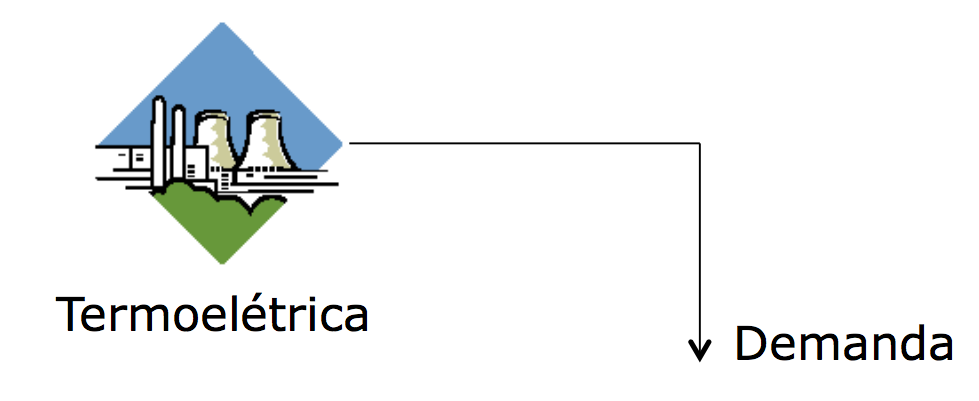
\includegraphics[width=7cm,height=3cm]{CO2.png}
\end{frame}

\begin{frame}
	\frametitle{Função Objetivo}
	É a \alert{expressão matemática do critério de otimização} descrita em termos das \alert{variáveis de decisão} do problema.
	\begin{table}
		\caption{Classificação da FOB}
		\begin{tabular}{r l}
			\hline
			\hline
			\alert{Continuidade} & Contínua   \\
								 & Descontínua \\
								 & Discreta    \\
			\hline
			\alert{Modalidade}   & Unimodal   \\
							     & Multimodal \\
			\hline
			\alert{Convexidade}  & Côncava ou Convexa \\
							     & Côncava e Convexa \\
							     & Nem Côncava e Nem Convexa \\
			\hline
		\end{tabular}
	\end{table}
	Além disto, a FOB pode ser \alert{linear ou não linear} e \alert{Mono-objetivo ou Multi-objetivo}.
                                                \end{frame}

\begin{frame}
	\centering
	\only<1>
	{
	\frametitle{FOB Contínua em todos os pontos}
	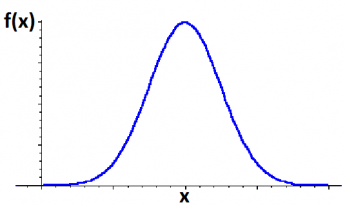
\includegraphics[width=8cm,height=5cm]{continua1.png}	
	}
	\only<2>
	{
	\frametitle{FOB Contínua em todos os pontos}
	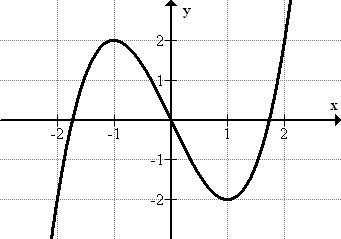
\includegraphics[width=8cm,height=5cm]{continua2.jpg}	
	}
	\only<3>
	{
	\frametitle{FOB Contínua, mas não diferenciável, em todos os pontos}
	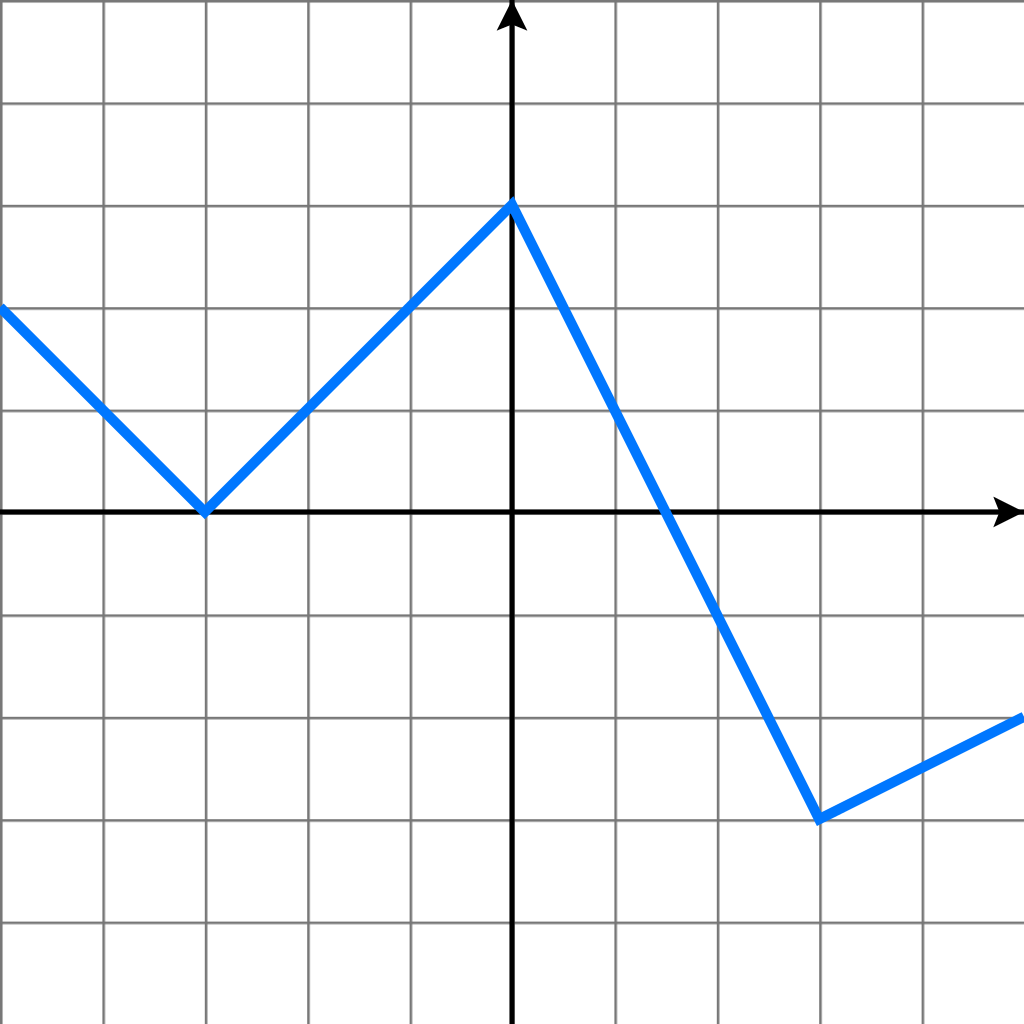
\includegraphics[width=8cm,height=5cm]{naodiferenciavel.png}	
	}
	\only<4>
	{
	\frametitle{FOB Descontínua}
	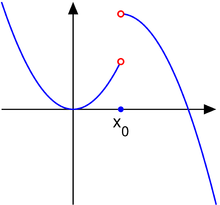
\includegraphics[width=8cm,height=5cm]{descontinua1.png}	
	}
	\only<5>
	{
	\frametitle{FOB Descontínua}
	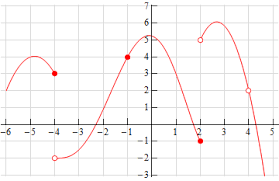
\includegraphics[width=8cm,height=5cm]{descontinua2.png}	
	}
	\only<6>
	{
	\frametitle{FOB Discreta}
	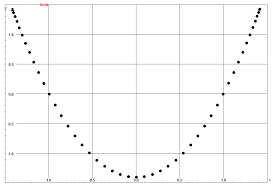
\includegraphics[width=8cm,height=5cm]{discreta1.png}	
	}
	\only<7>
	{
	\frametitle{FOB Discreta}
	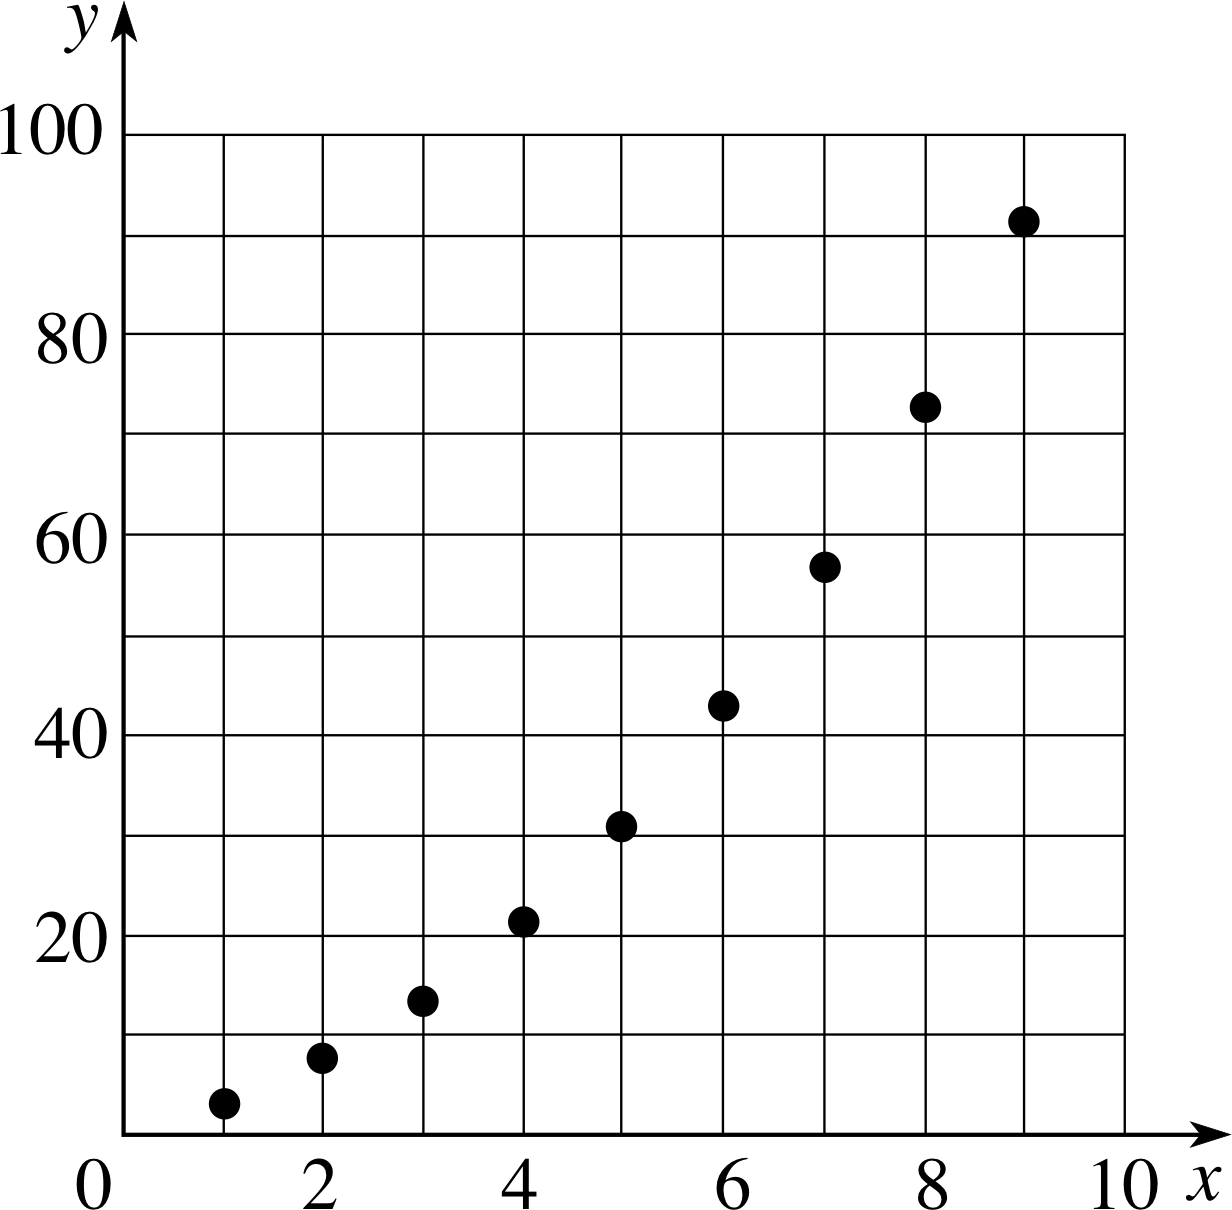
\includegraphics[width=8cm,height=5cm]{discreta2.png}	
	}
\end{frame}

\begin{frame}
	\centering
	\only<1>
	{
	\frametitle{Unimodal em 1 Dimensão}
	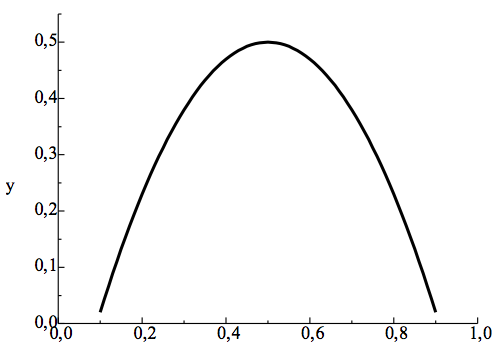
\includegraphics[width=8cm,height=5cm]{unimodal1.png}	
	}
	\only<2>
	{
	\frametitle{Unimodal em 2 Dimensões}
	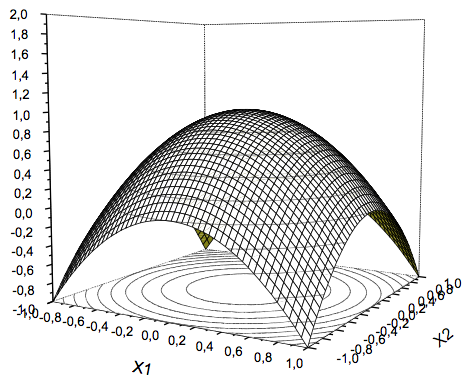
\includegraphics[width=8cm,height=5cm]{unimodal2.png}	
	}
	\only<3>
	{
	\frametitle{Multimodal em 1 Dimensão}
	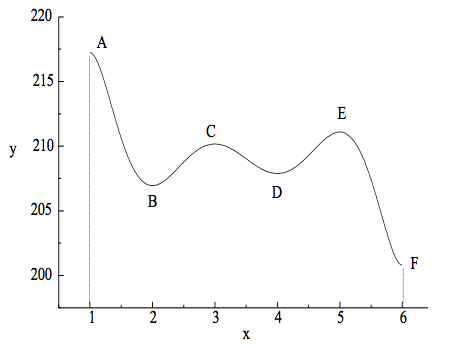
\includegraphics[width=8cm,height=5cm]{multimodal1.png}	
	}
	\only<4>
	{
	\frametitle{Multimodal em 2 Dimensões}
	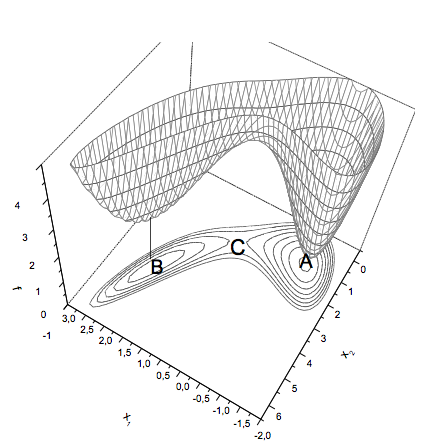
\includegraphics[width=8cm,height=5cm]{multimodal2.png}	
	}
\end{frame}

\begin{frame}
	\frametitle{Funções Multimodais}
	\centering
	\begin{columns}
		\begin{column}{0.15\textwidth}
			
\includegraphics[width=2cm,height=3cm]{duvida.jpg}
		\end{column}
		\begin{column}{0.6\textwidth}
			Sendo o objetivo a minimização da função $f(x_1,x_2)$ apresentada. Quantas soluções existem?
		\end{column}
		\only<3>
		{
			\begin{column}{0.35\textwidth}
				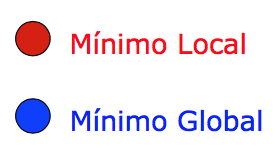
\includegraphics[width=2.5cm,height=1cm]{multimodal4.png}	
			\end{column}
		}		
	\end{columns}
	\only<1>
	{
		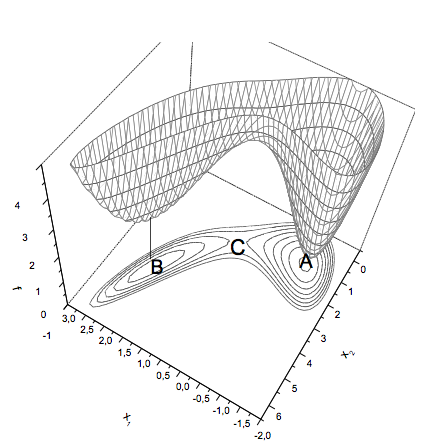
\includegraphics[width=8cm,height=5cm]{multimodal2.png}	
	}
	\only<2->
	{
		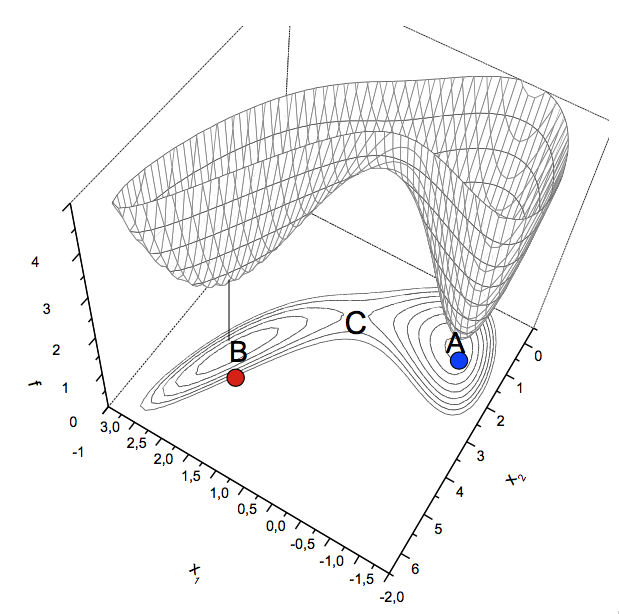
\includegraphics[width=8cm,height=5cm]{multimodal3.png}	
	}	
\end{frame}

\begin{frame}
	\centering
	\only<1>
	{
	\frametitle{Função Côncava}
	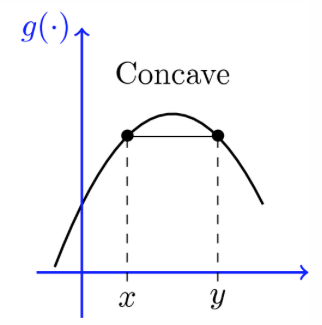
\includegraphics[width=8cm,height=5cm]{concava.png}	
	}
	\only<2>
	{
	\frametitle{Função Convexa}
	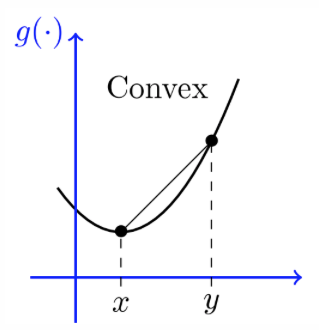
\includegraphics[width=8cm,height=5cm]{convexa.png}	
	}
	\only<3>
	{
	\frametitle{Função Côncava/Convexa}
	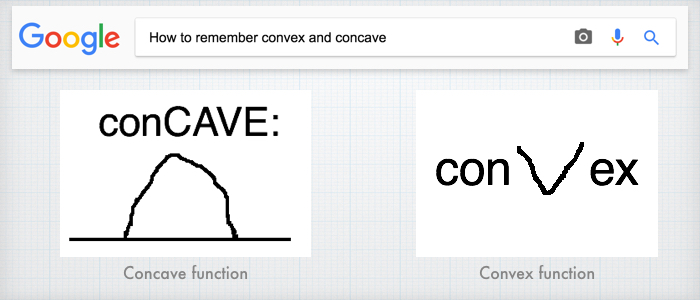
\includegraphics[width=10cm,height=5cm]{concaveandconvexgoogle.jpg}	
	}
	\only<4>
	{
	\frametitle{Nem Côncava, Nem Convexa }
	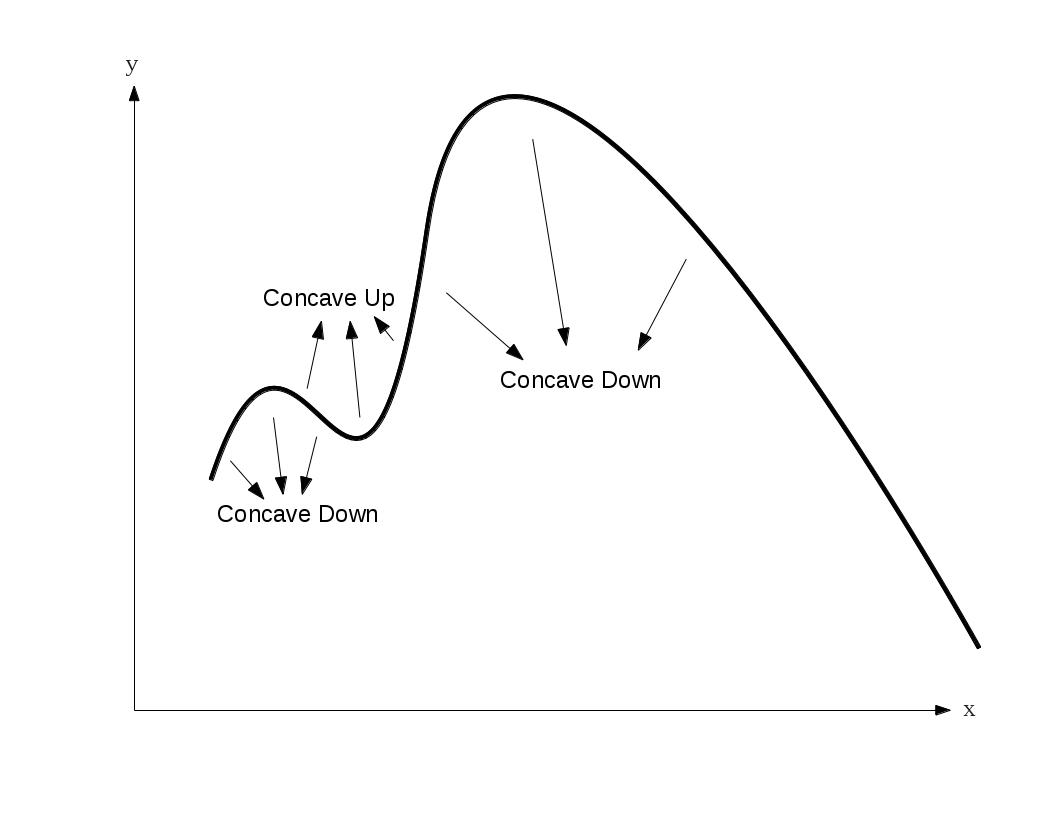
\includegraphics[width=8cm,height=5cm]{nemconcavonemconvexo.jpg}	
	}
\end{frame}

\begin{frame}
	\centering
	\only<1>
	{
		\frametitle{Função Côncava - Garantia de Ótimo Global?}
		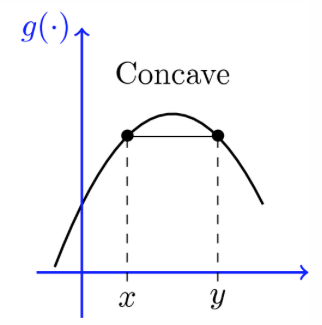
\includegraphics[width=8cm,height=5cm]{concava.png}	
	}
	\only<2>
	{
		\frametitle{Função Côncava - Garantia de Ótimo Global?}
		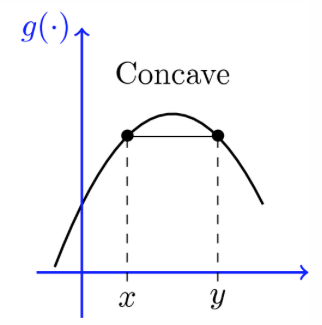
\includegraphics[width=8cm,height=5cm]{concava.png}	
		
\includegraphics[width=1cm,height=1cm]{sim.png}
	}
	\only<3>
	{
		\frametitle{Função Convexa - Garantia de Ótimo Global?}
		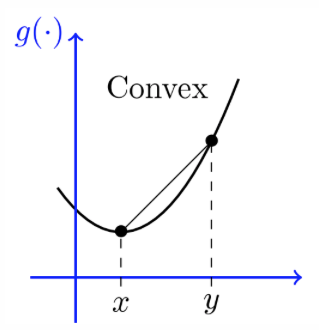
\includegraphics[width=8cm,height=5cm]{convexa.png}	
	}
	\only<4>
	{
		\frametitle{Função Convexa - Garantia de Ótimo Global?}
		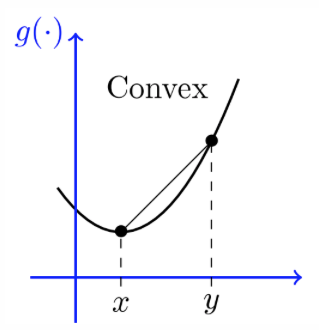
\includegraphics[width=8cm,height=5cm]{convexa.png}	
		
\includegraphics[width=1cm,height=1cm]{sim.png}
	}	
	\only<5>
	{
		\frametitle{Nem Côncava, Nem Convexa - Garantia de Ótimo Global? }
		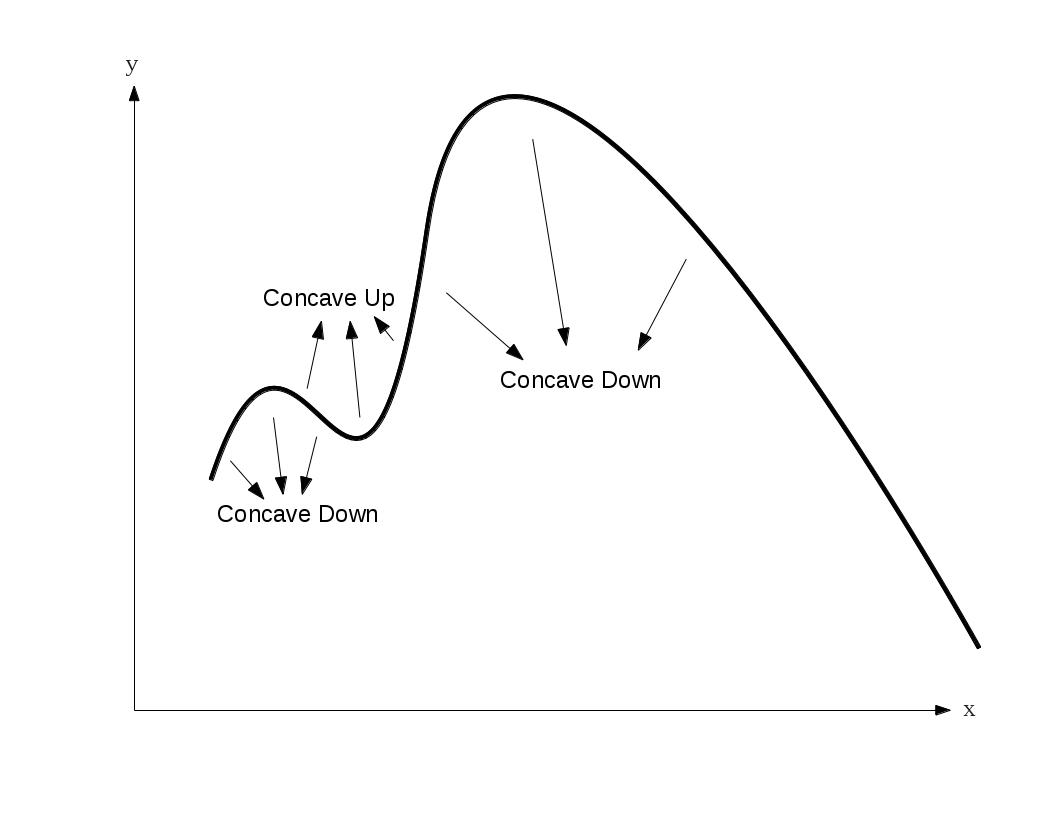
\includegraphics[width=8cm,height=5cm]{nemconcavonemconvexo.jpg}	
	}
	\only<6>
	{
		\frametitle{Nem Côncava, Nem Convexa - Garantia de Ótimo Global? }
		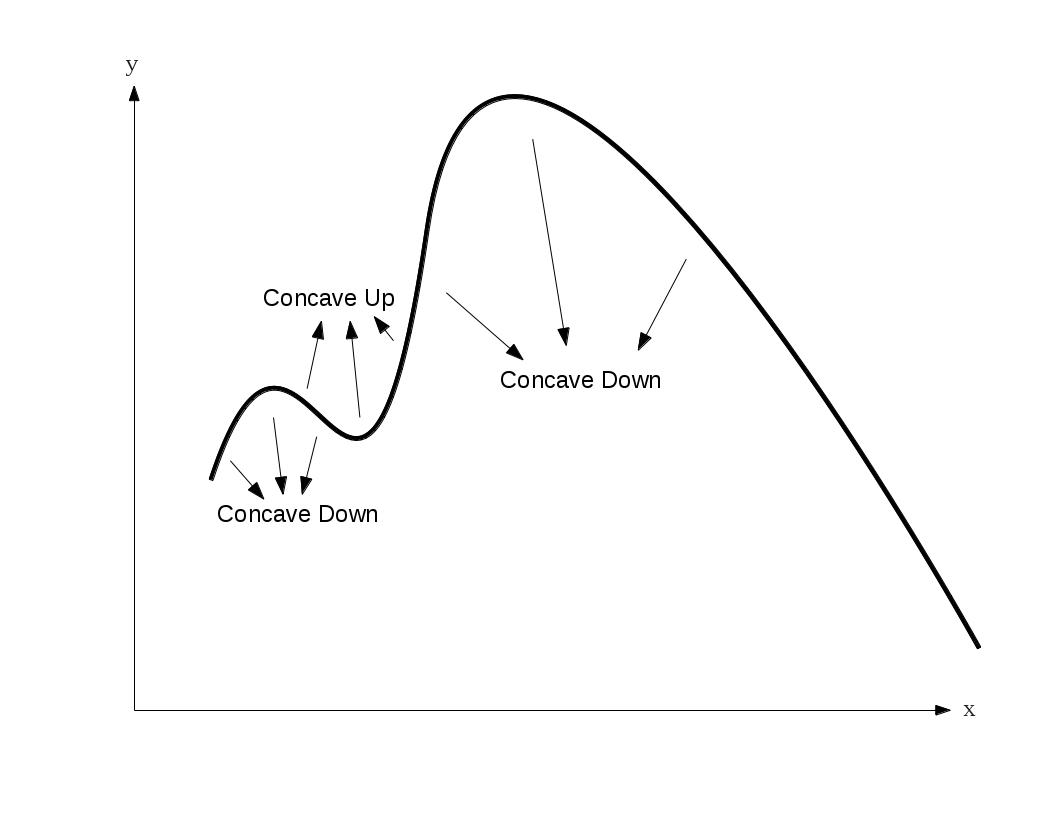
\includegraphics[width=8cm,height=5cm]{nemconcavonemconvexo.jpg}	
		
\includegraphics[width=1cm,height=1cm]{nao.png}
	}
\end{frame}

\begin{frame}
	\frametitle{Examinando a Convexidade/Concavidade}
	\begin{table}
		\begin{tabular}{c}
			A Função é \\
		\end{tabular}
		\begin{tabular}{c c c c}
			\hline
			\hline
			Côncava & Estritamente & Convexa & Estritamente \\
				    & Côncava      &         & Convexa      \\
			\hline
			$f''(x) \le 0$ & $f''(x) < 0$ & $f''(x) \ge 0$ & $f''(x) > 0$ \\
			\hline
			\hline
		\end{tabular}
	\end{table}
\end{frame}

\begin{frame}
	\frametitle{Funções Multivariadas}
	\centering
	\only<1>
	{
	$
	H = \begin{bmatrix}
	\frac{\partial ^2 f(x)}{\partial x_1^2} & \frac{\partial ^2 f(x)}{\partial x_1 \partial x_2} & \cdots  & \frac{\partial ^2 f(x)}{\partial x_1 \partial x_n}\\ 
	\frac{\partial ^2 f(x)}{\partial x_2 \partial x_1} & \frac{\partial ^2 f(x)}{\partial x_2^2} & \cdots  & \frac{\partial ^2 f(x)}{\partial x_2 \partial x_n}\\ 
	 \vdots & \vdots & \vdots & \vdots \\ 
	\frac{\partial ^2 f(x)}{\partial x_n \partial x_1} & \frac{\partial ^2 f(x)}{\partial x_n \partial x_2} & \cdots & \frac{\partial ^2 f(x)}{\partial x_1^2} \\
	\end{bmatrix}
	$
	}
	\only<2>
	{
	$
	H = \begin{bmatrix}
	\cellcolor{red!45} \frac{\partial ^2 f(x)}{\partial x_1^2} & \frac{\partial ^2 f(x)}{\partial x_1 \partial x_2} & \cdots  & \frac{\partial ^2 f(x)}{\partial x_1 \partial x_n}\\ 
	\frac{\partial ^2 f(x)}{\partial x_2 \partial x_1} & \frac{\partial ^2 f(x)}{\partial x_2^2} & \cdots  & \frac{\partial ^2 f(x)}{\partial x_2 \partial x_n}\\ 
	 \vdots & \vdots & \vdots & \vdots \\ 
	\frac{\partial ^2 f(x)}{\partial x_n \partial x_1} & \frac{\partial ^2 f(x)}{\partial x_n \partial x_2} & \cdots & \frac{\partial ^2 f(x)}{\partial x_1^2} \\
	\end{bmatrix}
	$
	}
	\only<3>
	{
	$
	H = \begin{bmatrix}
	\cellcolor{red!45} \frac{\partial ^2 f(x)}{\partial x_1^2} & \cellcolor{red!45} \frac{\partial ^2 f(x)}{\partial x_1 \partial x_2} & \cdots  & \frac{\partial ^2 f(x)}{\partial x_1 \partial x_n}\\ 
	\cellcolor{red!45} \frac{\partial ^2 f(x)}{\partial x_2 \partial x_1} & \cellcolor{red!45} \frac{\partial ^2 f(x)}{\partial x_2^2} & \cdots  & \frac{\partial ^2 f(x)}{\partial x_2 \partial x_n}\\ 
	 \vdots & \vdots & \vdots & \vdots \\ 
	\frac{\partial ^2 f(x)}{\partial x_n \partial x_1} & \frac{\partial ^2 f(x)}{\partial x_n \partial x_2} & \cdots & \frac{\partial ^2 f(x)}{\partial x_1^2} \\
	\end{bmatrix}
	$
	}
	\only<4>
	{
	$
	H = \begin{bmatrix}
	\cellcolor{red!45} \frac{\partial ^2 f(x)}{\partial x_1^2} & \cellcolor{red!45} \frac{\partial ^2 f(x)}{\partial x_1 \partial x_2} & \cellcolor{red!45} \cdots  & \cellcolor{red!45} \frac{\partial ^2 f(x)}{\partial x_1 \partial x_n}\\ 
	\cellcolor{red!45} \frac{\partial ^2 f(x)}{\partial x_2 \partial x_1} & \cellcolor{red!45} \frac{\partial ^2 f(x)}{\partial x_2^2} & \cellcolor{red!45} \cdots  & \cellcolor{red!45} \frac{\partial ^2 f(x)}{\partial x_2 \partial x_n}\\ 
	\cellcolor{red!45} \vdots & \cellcolor{red!45} \vdots & \cellcolor{red!45} \vdots & \cellcolor{red!45} \vdots \\ 
	\cellcolor{red!45} \frac{\partial ^2 f(x)}{\partial x_n \partial x_1} & \cellcolor{red!45} \frac{\partial ^2 f(x)}{\partial x_n \partial x_2} & \cellcolor{red!45} \cdots & \cellcolor{red!45} \frac{\partial ^2 f(x)}{\partial x_1^2} \\
	\end{bmatrix}
	$
	}
	 
	\begin{itemize}
	\item A função multivariada é \alert{convexa} se a sua matriz Hessiana é \alert{positiva semidefinda}.
	\item A função multivariada é \alert{côncava} se a sua matriz Hessiana é \alert{negativa semidefinda}.
	\item Critério de Sylvester: Todos os menores principais devem ser positivos (convexa) ou negativos (côncava).	
	\end{itemize}
\end{frame}

\begin{frame}
	\frametitle{Examine a convexidade da seguinte função}
	\only<1>
	{
	\begin{exampleblock}{$f(x)=-3x^2-4x+4$} 
		\begin{itemize}
		\item[] $f'(x) = -6x - 4$
		\item[] $f''(x) = -6 < 0$ para todo x
		\item[] A função é estritamente côncava.
		\end{itemize}
	\end{exampleblock}
	}
	\only<2>
	{
	\begin{exampleblock}{$f(x)=e^{x^2}$} 
		\begin{itemize}
		\item[] $f'(x) = 2xe^{x^2}$
		\item[] $f''(x) = 4x^2e^{x^2}+2e^{x^2} > 0$ para todo x
		\item[] A função é estritamente convexa.
		\end{itemize}
	\end{exampleblock}
	}	
	\only<3>
	{
	\begin{exampleblock}{$f(x_1,x_2,x_3)=6x_1^2+4x_2^2+2x_3^2+6x_1x_2-3x_1-4x_2+20$} 
		\begin{itemize}
		\item[] 
				$ H = \begin{bmatrix}
									  12 & 6 & 0 \\
									   6  & 8 & 0 \\
									   0  & 0 & 4 \\
					   \end{bmatrix} 
				$
		\item[] 
				$ \begin{vmatrix}
							     12
				  \end{vmatrix} > 0 
				$
		\item[] 
				$ \begin{vmatrix}
									  12 & 6 \\
									   6 & 8 \\
				   \end{vmatrix} = 60 > 0 
				$		
		\item[]
				$ \begin{vmatrix}
									  12 & 6 & 0 \\
									   6  & 8 & 0 \\
									   0  & 0 & 4 \\
				   \end{vmatrix} = 240 > 0 
				$
		\item[] Matriz definida positiva. Função estritamente convexa.		
		\end{itemize}
	\end{exampleblock}
	}		
\end{frame}

\begin{frame}
	\frametitle{Região de Solução nem Côncava nem Convexa}
	\centering
	\only<1>
	{
	O problema tem várias soluções, porém a garantia da otimalidade global é comprometida.
	\begin{table}
		\begin{tabular}{c}
			Dependendo da região de solução e do tamanho do problema \\
			\includegraphics[width=2cm,height=2cm]{seta_baixo.png} \\
			Otimalidade Global \\
			\includegraphics[width=2.5cm,height=2.5cm]{agulha_palheiro.jpg} \\
			Agulha no Palheiro \\
		\end{tabular}
	\end{table}
	}
	\only<2>
	{
	\begin{alertblock}{Encontre a solução ótima para o seguinte problema de otimização:}
		\begin{itemize}
		\item[] Max $F(x,y) = x^2 + y^2 + 25( \sin^2 x + \sin^2 y)$
		\item[] s.a.
		\item[] $ -6 \le x \le 6$
		\item[] $ -6 \le y \le 6$
		\end{itemize}
	\end{alertblock}
	\includegraphics[width=4.5cm,height=3.5cm]{easyhard.jpg}
	\includegraphics[width=3.5cm,height=2cm]{interrogacao.jpg}
	}
	
\end{frame}


\begin{frame}
	\frametitle{Egg Crate Function} 
	\centering
	\includegraphics[width=10cm,height=7cm]{eggcrate.png}
\end{frame}

\begin{frame}[fragile]
	\frametitle{Egg Crate Function}
	\begin{block}{Código em Matlab}
		\begin{lstlisting}
clear all; close all; clc;

x = [-6:0.1:6]; y = [-6:0.1:6];
[X,Y] = meshgrid(x,y);

egg_crate = @(x,y) x.^2 + y.^2 ...
    + 25*( sin(x).^2 + sin(y).^2 );
Z = egg_crate(X,Y);

grafico=mesh(x,y,Z); colormap(hsv);

title('Eggcrate Function - 3D');
xlabel('x','FontSize',14); 
ylabel('y','FontSize',14); 
zlabel('f(x,y)','FontSize',14);
grafico.Parent.FontSize = 14;
		\end{lstlisting}
	\end{block}	
\end{frame}

\begin{frame}
	\only<1>
	{
	\frametitle{Egg Crate Function}
	\centering
	\includegraphics[width=10cm,height=7cm]{eggcrate_max.png}
	}
	\only<2>
	{
	\frametitle{Egg Crate Function - Máximos Locais e Globais} 	
	\centering
	\includegraphics[width=10cm,height=7cm]{egg_crate_2d.png}
	}	
\end{frame}

\begin{frame}[fragile]
	\frametitle{Egg Crate Function}
	\begin{block}{Código em Matlab}
		\begin{lstlisting}
clear all; close all; clc;

x = [-6:0.1:6]; y = [-6:0.1:6];
[X,Y] = meshgrid(x,y);

egg_crate = @(x,y) x.^2 + y.^2 ...
    + 25*( sin(x).^2 + sin(y).^2 );
Z = egg_crate(X,Y);

grafico=mesh(x,y,Z); colormap(hsv);

title('Eggcrate Function - 3D');
xlabel('x','FontSize',14); 
ylabel('y','FontSize',14); 
zlabel('f(x,y)','FontSize',14);
grafico.Parent.FontSize = 14;
		\end{lstlisting}
	\end{block}	
\end{frame}

\begin{frame}
	\frametitle{Região de Solução nem Côncava nem Convexa}
	\centering
	\begin{alertblock}{Ackley Function (caso bi-dimensional):}
		\begin{itemize}
		\item[] Max $F(x,y) = -20e^{-0.2\sqrt{0.5(x^2+y^2)}} - e^{0.5(\cos 2 \pi x + \cos 2 \pi y)} + e + 20$
		\item[] s.a.
		\item[] $ -32 \le x \le 32$
		\item[] $ -32 \le y \le 32$
		\end{itemize}
	\end{alertblock}	
	É uma função não convexa muito utilizada para testar a performance de algoritmos de otimização.
\end{frame}

\begin{frame}
	\frametitle{Ackley Function}
	\only<1>
	{
	\centering
	\includegraphics[width=10cm,height=7cm]{ackley1.png}
	}
	\only<2>
	{
	\centering
	\includegraphics[width=10cm,height=7cm]{ackley2.png}
	}	
	\only<3>
	{
	\centering
	\includegraphics[width=10cm,height=7cm]{ackley3.png}
	}
	\only<4>
	{
	\centering
	\includegraphics[width=10cm,height=7cm]{ackley4.png}
	}	
\end{frame}

\begin{frame}
	\frametitle{Restrições}
	São os \alert{limites} impostos pelas leis/regras que regem o modelo. Há 3 tipos de restrições:
	\begin{itemize}
	\item {Restrições de \underline{igualdade}: $\color{red} h(x) = 0$}
		\begin{itemize}
		\item[] São as equações do próprio modelo matemático.
		\end{itemize}
	\item {Restrições de \underline{desigualdade}: $\color{red} g(x) \le 0$}
		\begin{itemize}
		\item[] São os limites impostos às funções do modelo matemático.
		\end{itemize}
	\item {Restrições de \underline{canalização}: $\color{red} \text{xmin} \le x \le \text{xmax}$} 
		\begin{itemize}
		\item[] São os limites impostos às variáveis de decisão.
		\end{itemize}
	\end{itemize}
	As restrições podem ser \alert{lineares} e/ou \alert{não lineares}.
\end{frame}

\begin{frame}
	\frametitle{Restrições - Exemplo}
	\only<1>
	{
		\frametitle{Restrições - Exemplo}
		\begin{block}{Parabolóide Elíptico - Superfície Quadrática}
			\begin{itemize}
			\item Maximizar $Z$
			\item Sujeito a:
			\item $Z = -2x^2 - 2y^2 + 4$
			\end{itemize}
		\end{block}
	}
	\only<2>
	{ 
		\frametitle{Restrições - Exemplo}
		\includegraphics[width=10cm,height=7cm]{restricoes1.png}
	}
	\only<3>
	{ 
		\frametitle{Restrições - Exemplo}
		\includegraphics[width=10cm,height=7cm]{restricoes2.png}
	}
	\only<4>
	{
		\frametitle{Restrições - Exemplo}
		\begin{block}{Parabolóide Elíptico - Superfície Quadrática}
			\begin{itemize}
			\item Maximizar $Z$
			\item Sujeito a:
			\item $Z = -2x^2 - 2y^2 + 4$
			\item $\color{red} x \le 1 $
			\item $\color{red} y - 1.5x + 0.75 \le 0$
			\item $\color{red} y \ge 0$
			\end{itemize}
		\end{block}
	}	
	\only<5>
	{ 
  	    \frametitle{Restrições - Exemplo - Região Viável}
		\includegraphics[width=10cm,height=7cm]{restricoes3.png}
	}
	\only<6>
	{ 
  	    \frametitle{Restrições - Exemplo - Região Viável}
		\includegraphics[width=10cm,height=7cm]{restricoes4.png}
	}
\end{frame}

\begin{frame}
	\frametitle{Formulação Geral de um Problema de Otimização}
	\only<1>
	{
		\begin{itemize}
		\item[] 
				\begin{equation*}
					\text{Minimizar ou Minimizar } f\text{(} \mathbf{x} \text{)}
				\end{equation*}
		\item[] Sujeito a:
		\item[] 
				\begin{equation*}
					\begin{matrix}
						\mathbf{h}( \mathbf{x} )=0   \\ 
						\mathbf{g}( \mathbf{x} ) (\le, \ge) 0  \\ 
						\mathbf{x_{min}} \le \mathbf{x} \le \mathbf{x_{max}} \\ 
					\end{matrix}
				\end{equation*}
		\end{itemize}
	}
	\only<2>
	{
		\begin{itemize}
		\item[] 
				\begin{equation*}
					\text{Minimizar ou Minimizar } f\text{(} \overset{\includegraphics[width=0.4cm,height=0.4cm]{redstar.png}
					}{\mathbf{x}} \text{)}
				\end{equation*}
		\item[] Sujeito a:
		\item[] 
				\begin{equation*}
					\begin{matrix}
					\mathbf{h}(\mathbf{\overset{\includegraphics[width=0.4cm,height=0.4cm]{redstar.png}
									}{\mathbf{x}}})=0                             & (\mathbf{\lambda_1}) \includegraphics[width=0.4cm,height=0.4cm]{bluestar.png}\\ 
					\mathbf{g}(\mathbf{\overset{\includegraphics[width=0.4cm,height=0.4cm]{redstar.png}
									}{\mathbf{x}}})(\le, \ge)) 0                  & (\mathbf{\lambda_2})  \includegraphics[width=0.4cm,height=0.4cm]{bluestar.png}\\ 
					\mathbf{x_{min}} \le \mathbf{\overset{\includegraphics[width=0.4cm,height=0.4cm]{redstar.png}
									}{\mathbf{x}}} \le \mathbf{x_{max}} & (\mathbf{\lambda_3, \lambda_4}) \includegraphics[width=0.4cm,height=0.4cm]{bluestar.png}\\ 
					\end{matrix}
				\end{equation*}
		\item[]
				\begin{table}
					\begin{tabular}{| r l |}
							\hline
							\includegraphics[width=0.4cm,height=0.4cm]{redstar.png} & Variáveis Primais \\
							\hline
							\includegraphics[width=0.4cm,height=0.4cm]{bluestar.png} & Variáveis Duais \\
							\hline
					\end{tabular}
				\end{table}
		\item[] 
				\begin{table}
					\begin{tabular}{c}
						\cellcolor{yellow} Formulação pode ser \alert{LINEAR} ou \alert{NÃO LINEAR}
					\end{tabular}
				\end{table}
		\end{itemize}
	}
\end{frame}

\begin{frame}
	\frametitle{Exemplo de Problema de Otimização}
	\only<1->
	{
		\includegraphics[width=11cm,height=5.5cm]{exemplo.png}
	}
	\only<2>
	{
		\begin{table}
			\begin{tabular}{c}
				\Large \color{blue} CURIOSIDADES
			\end{tabular}
			\begin{tabular}{c c}
				\multirow{3}{*}{ \includegraphics[width=1.5cm,height=1.5cm]{horror.jpg} } 
								     & \cellcolor{green} Resolução do problema de gerenciamento da carteira \\
									 & \cellcolor{green} de um fundo de pensão holandes utilizando PL: \\
						             & \cellcolor{green} 12,5 milhoes de restrições e 25 milhões de variáveis \\
			\end{tabular}
		\end{table}
	}
\end{frame}

\begin{frame}
\Huge{\centerline{Fim}}
\end{frame}

%----------------------------------------------------------------------------------------

\end{document} 